\section{Enforcement Proxy}
\label{sec:proxy}

The enforcement proxy intercepts every tool call between the LLM agent and tool executors, evaluating it against policies before allowing execution.

\subsection{Proxy Workflow}

\begin{figure}[t]
  \centering
  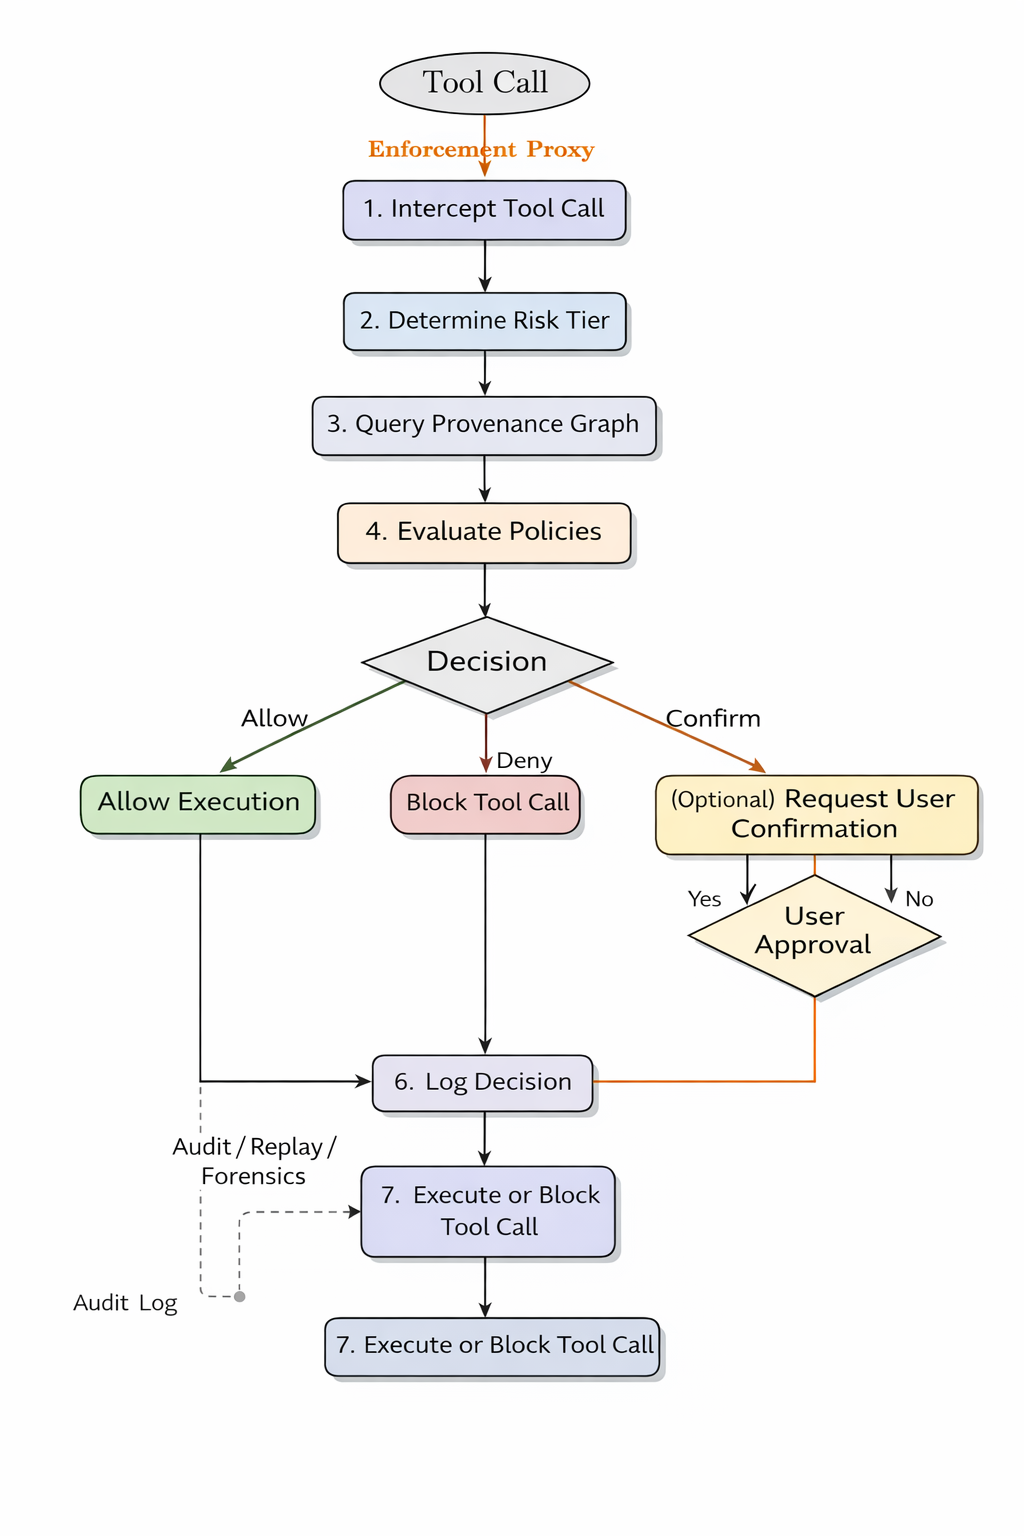
\includegraphics[width=\columnwidth]{figures/proxy_flow.png}
  \caption{Enforcement Proxy Workflow. Each tool call passes through seven decision stages before execution.}
  \label{fig:proxy}
\end{figure}

The proxy executes a seven-stage pipeline for every proposed tool call (Fig.~\ref{fig:proxy}):
\textbf{(1)~Interception} of the tool invocation;
\textbf{(2)~Argument pre-processing}---a canonicalization pass decodes arguments through nine encoding schemes (Unicode NFKD, hex escapes, octal, Base64, pure hex, ROT13, URL percent-encoding with double-decode, binary strings, HTML entities) and flags suspicious structural patterns (path traversal, shell metacharacters). \emph{Critically, this stage marks flagged arguments as UNTRUSTED rather than short-circuiting the pipeline.} This ensures the provenance and policy stages are always consulted, enabling ablation studies and preventing the canonicalization pass from becoming a single point of failure;
\textbf{(3)~Provenance resolution} via the three-stage pipeline (Section~\ref{sec:policies}), incorporating any untrusted labels injected by Stage~2;
\textbf{(4)~Policy evaluation} in priority order (Algorithm~\ref{alg:policy}), with provenance information from Stages~2--3 combined into a single \texttt{has\_untrusted\_args} signal;
\textbf{(5)~User confirmation} if the matched rule returns REQUIRE\_CONFIRMATION;
\textbf{(6)~Decision logging} in an append-only, SHA-256--chained audit ledger;
\textbf{(7)~Execution or denial}---approved calls proceed; denied calls return errors to the agent.

\subsection{Policy Evaluation Algorithm}

Algorithm~\ref{alg:policy} shows the core logic. Rules are evaluated top-to-bottom (\emph{first-match semantics}), conditions combine with AND logic (\emph{conjunctive conditions} with short-circuit evaluation), and unmatched HIGH/CRITICAL tools default to REQUIRE\_CONFIRMATION (\emph{fail-safe defaults}).

\begin{algorithm}[t]
\caption{Policy Evaluation Algorithm}
\label{alg:policy}
\begin{algorithmic}[1]
\Procedure{EvaluatePolicy}{$call, policy, provGraph$}
  \State $tool \gets call.tool$; $args \gets call.args$
  \For{$rule$ in $policy.rules$}
    \If{\Call{ToolMatches}{$tool, rule.tools$}}
      \If{\Call{AllConditionsMet}{$rule, args, provGraph$}}
        \State \Return $rule.action$  \Comment{First match wins}
      \EndIf
    \EndIf
  \EndFor
  \State \Return \Call{DefaultAction}{$tool$}
\EndProcedure
\Procedure{AllConditionsMet}{$rule, args, provGraph$}
  \For{$cond$ in $rule.conditions$}
    \If{NOT \Call{EvalCond}{$cond, args, provGraph$}}
      \State \Return \texttt{false}
    \EndIf
  \EndFor
  \State \Return \texttt{true}
\EndProcedure
\end{algorithmic}
\end{algorithm}

The algorithm is intentionally simple: complex reasoning about information lineage is handled by the provenance tracker, while decision logic is straightforward rule matching. Policy evaluation completes in median 0.06\,ms; provenance queries take median 0.82\,ms---both negligible compared to LLM inference latency (500--2000\,ms).

\subsection{Auditability and Replay}

The proxy's determinism enables \emph{replay verification}: given a prior decision log, identical tool-call/provenance inputs, and the same temporal/rate-limit state, administrators can re-execute decisions and confirm identical results. Decision logs are encrypted at rest and tamper-evident via SHA-256 hash chaining. The proxy integrates with agents via Python decorators or as an HTTP/gRPC server, requiring no modifications to agent internals.
